%\title{ \huge \bfseries Q-ant \& Q-gen}
%----------------------------------------------------------------------------------------
%	PACKAGES AND OTHER DOCUMENT CONFIGURATIONS
%----------------------------------------------------------------------------------------

\documentclass[10pt]{article}
\usepackage[english]{babel}
\usepackage[utf8]{inputenc}
\usepackage{amsmath}
\usepackage{graphicx}
\usepackage[colorinlistoftodos]{todonotes}
\usepackage{hyperref}
\usepackage{booktabs,array}
\usepackage{tabto}
\usepackage{systeme, mathtools}
\usepackage{amssymb}
%\usepackage{varioref}
\usepackage{float}
\floatstyle{plaintop}
\restylefloat{table}
\usepackage[title]{appendix}
\usepackage[margin=3cm]{geometry}
\usepackage{enumitem}
\usepackage{algorithm}
\usepackage[noend]{algpseudocode}
%\usepackage{floatrow}
%\floatsetup[table]{capposition=top}
\usepackage[tableposition=top]{caption}
\usepackage{tabularx}
%\captionsetup[table]{position = top}   %% or bottom
%\usepackage{tabls}
\usepackage{csquotes}
\MakeOuterQuote{"}

\makeatletter
\def\BState{\State\hskip-\ALG@thistlm}
\makeatother
\renewcommand{\floatpagefraction}{.9}
%\renewcommand{\textfraction}{0.01} 
%\usepackage[autostyle]{csquotes}
%\MakeOuterQuote{"}
\begin{document}

\begin{titlepage}

\newcommand{\HRule}{\rule{\linewidth}{0.5mm}} % Defines a new command for the horizontal lines, change thickness here

\center % Center everything on the page
 
%----------------------------------------------------------------------------------------
%	HEADING SECTIONS
%----------------------------------------------------------------------------------------

\textsc{\LARGE Università degli studi di Milano-Bicocca}\\[1cm] % Name of your university/college
\textsc{\Large Text Mining and Search}\\[0.3cm] % Major heading such as course name
\textsc{\large Final Project}\\[0.1cm] % Minor heading such as course title

%----------------------------------------------------------------------------------------
%	TITLE SECTION
%----------------------------------------------------------------------------------------
\HRule \\[0.4cm]
%\maketitle
{ \huge \bfseries Meetup Topics: \\ \vspace{0.2cm}{\Large Classify Meetup.com Event Descriptions}}\\[0.4cm] % Title of your document
\HRule \\[1.5cm]
 
%----------------------------------------------------------------------------------------
%	AUTHOR SECTION
%----------------------------------------------------------------------------------------

\large
\emph{Authors:}\\
Dario Bertazioli - 847761 - d.bertazioli@campus.unimib.it \\   % Your name
Fabrizio D'Intinosante - 838866 - f.dintinosante@campus.unimib.it \\
Massimiliano Perletti - 847548 - m.perletti2@campus.unimib.it\\[1cm] % Your name
% If you don't want a supervisor, uncomment the two lines below and remove the section above
%\Large \emph{Author:}\\
%John \textsc{Smith}\\[3cm] % Your name

%----------------------------------------------------------------------------------------
%	DATE SECTION
%----------------------------------------------------------------------------------------

{\large \today}\\[2cm] % Date, change the \today to a set date if you want to be precise

%----------------------------------------------------------------------------------------
%	LOGO SECTION
%----------------------------------------------------------------------------------------


\includegraphics[scale=0.15]{figs/logo_uni.png}\\[1cm] % Include a department/university logo - this will require the graphicx package

%----------------------------------------------------------------------------------------

\vfill % Fill the rest of the page with whitespace

\end{titlepage}
\vspace*{5cm}
\begin{abstract}
The following project aims to implement a text classification pipeline for the Meetup events description. 
Within the Meetup platform, every organized event needs to be manually tagged by the organizers to allow the platform's recommendation system to suggest the event to users based on their interests.
In this context, a system that suggests to organizers how to label their event based on how it was described by them would be a useful tool.
The text classification task is well known in literature and involves a series of operations and tricks, starting from the preprocessing of the texts up to the text representation. 
Our goal was to find the best combination of preprocessing and text representation to be submitted to the best classifier, based on the classification performance, to maximize some performance evaluation metrics.
\end{abstract}

\newpage
\tableofcontents
\newpage
\section{Introduction \label{sec:intro}}
Meetup is a platform created in 2002 with the purpose to get people in touch with others in real life. Once completed the registration process, users can:
\begin{itemize}
\item choose their \textbf{interests}: they subscribe to some pre-fill topics from the application to "warm" the recommendation system. 
These topics concern a lot of contexts, ranging from professional to "every-day" areas, like social events;
\item subscribe to local \textbf{groups}: after choosing the topic of interests, the recommendation system suggests the users with a series of local or not local groups. 
In this way, users could meet people who share the same hobbies. In the case in which users can’t find their topics of interest in the area, Meetup suggests creating a group that interest themselves, adding people that show the same interest;
\item participate in \textbf{events}: local groups organize events or meetings that concern topics in question. When a local group plans the event, users can see it on their homepage; in addition, they can decide to share their participation, in which they can suggest inviting some guests, or their absence. The app allows picking some filters to find other groups and topics.
\end{itemize}
The main focus in the whole application is the “group”, as a result of social aggregation. 
The variation of groups depends on considered topics:
\begin{itemize}
\item \textbf{socialization} groups, with the main aim of doing fun activities with other people; they can also organize dating events;
\item \textbf{professional} groups, to promote professional networking through workshops or meetings;
\item \textbf{creative} group, purposing activities such as team projects to practice different arts and hobbies. 
\end{itemize}
To sum up, the aim of Meetup is helping people to grow up and achieve their purposes through real connections. 
Nowadays, Meetup is available in 186 countries and it counts for over 40 million members, among which there are more than 320k online groups with an average of 12k events per day. 


\paragraph{Project Goals:}
The project aims is to perform a text (Single-Label Multi-Class, SLMC) classification task  starting from the descriptions and titles associated with the meetup.com events, to assign a category to the reference event.
Different text representation strategies , different types of pre-processing and two classification models, including Random Forest and a Neural Network, will be tested to check which of these may be the best application for the task in question.
Finally, an optimization pipeline will be addressed in order to identify a set of (possibly) optimal hyper-parameters to improve the performance of the final model.

\section{Dataset \label{sec:datasets}}
The dataset %obtained through REST API, %(non so se vogliamo menzionare o meno come è stato ottenuto o info in più)
is composed of 4 variables:
\begin{itemize}
\item \textit{description}: details of the event with all the information necessary for its development;
\item \textit{event\_id}: unique event code;
\item \textit{event\_name}: event title;
\item \textit{category}: label to identify the main topic related to the event.
\end{itemize}
A first step of removing missing values and duplicates is performed to obtain a dataset of about 134k observations.
As mentioned above, the purpose is to predict the category label of the event thanks to its description. Initially, the category can assume 32 different textual values (from sports, fitness, hobbies to music, writing, tech, etc.).
\begin{figure}
\centering
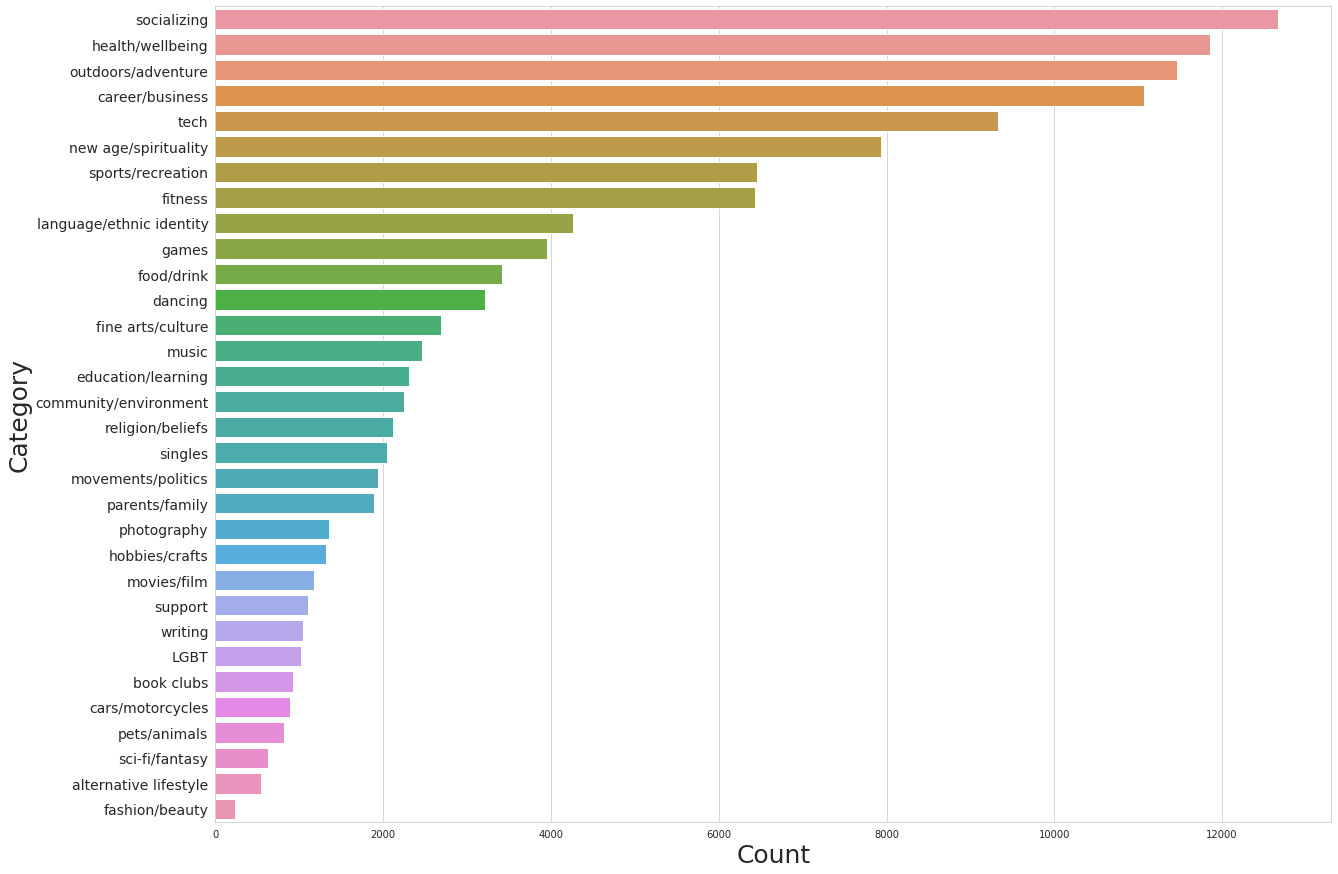
\includegraphics[scale=0.35]{figs/dist.png}
\caption{\label{fig:dist}Count-plot representing the number of events for each category.}
\end{figure}
In Fig.\ref{fig:dist}  the distribution of events in relation to their category is shown; it is possible to see how some categories are much more represented, compared to some that are probably referred to groups that share more particular interests.
Since some categories are under-represented and intuitively show some important similarity (common topics), a union of those categories has been applied with respect to the most similar topic (e.g. \textit{singles to socializing, book clubs to education/learning, etc..}). 
After this step, the final labels that will be predicted are 24.

\section{The Methodological Approach \label{sec:methods}}

The methodological approach followed in this project is articulated in three main phases: 
\begin{itemize}
\item a preprocessing phase, where suitable transformations are applied to the raw descriptions to provide a cleaner basis for the successive treatments;
\item a "text representation" phase, where some feature extractions are performed in such a way to provide a meaningful representation of the data under the "machine" perspective;
\item a classification phase, where the obtained text representations are fed in different classifiers to perform the objective task.
\end{itemize}
\subsection{Pre-processing \label{subsec:preprocessing}}
As usually happens in a typical text-mining pipeline, various pre-processing operations are applied to the raw text. 
In particular, the following transformations are applied in sequence:

\begin{itemize}
\item \textbf{Html Parsing}: exploiting the ever-green python package "Beautiful Soup"\footnote{\url{https://pypi.org/project/beautifulsoup4/}}, the raw descriptions, are found in an HTML, are parsed in such a way to remove the HTML tags and to retain the plain text. For instance, images and links, when occurring, are discarded.
\item \textbf{Emoji Removal}: the most-known emojis, i.e. those encoded in the python emoji package \footnote{\url{https://pypi.org/project/emoji/}}, are stripped since they are considered not relevant to the current classification task (the emoji would instead have been particularly relevant in other tasks, i.e. sentiment analysis/emotion detection).
\item \textbf{Language Detection}: the detection of the main language in a description is performed through the package "Polyglot" \footnote{\url{https://pypi.org/project/polyglot/}}, which provides a detector able to identify the language of possibly short texts, furthermore assigning a confidence score to the detection operation: whether the confidence is high, we tagged the description with its language, whereas when the detector is not able to reliably identify the main language the related description are tagged with an "Unknown Language" tag, and successively discarded.

\item \textbf{Language Translation}: as an experimental approach, non-anglophone languages are translated to English to provide a uniform linguistic panorama to the successive phases\footnote{However, after some experiments, we decided to simply only keep descriptions originally in English, since we noticed a degradation of performances after the translation. A minor part of descriptions are, therefore, discarded. The total number of description reduces to $\sim 120000$.}. 
Different translators are tested, such as the Google Translator API, the DeepL API, and the python-translate API (which collects translation from different providers like Microsoft, Yahoo etc.).

\item \textbf{Punctuation removal and normalization}: the punctuation is removed from the texts, which are successively normalized (accent removal, lower case normalization).

\item \textbf{Tokenization} and \textbf{stop-words removal}: the descriptions are tokenized (i.e. texts are split in single-words lists), and stop-words (frequently occurring and non-informative words, characteristics of the human language) are removed since considered not relevant to the final classification task.

\item \textbf{Stemming} and \textbf{Lemmatization}: two different processing operations are applied to the tokenized descriptions independently. Stemming is applied with the Porter Stemmer\footnote{Other stemmers are tested, such as the Snowball stemmer, providing similar results. The Porter Stemmer is therefore chosen as it usually represents the standard choice for this task.}.
Lemmatization is applied after a POS tagging. Both operations are performed exploiting the NLTK\footnote{\url{https://www.nltk.org/}} package.

\item \textbf{LDA clustering for "badwords" removal}: a further cleaning experiment is designed by means of the Latent Dirichlet Allocation~\cite{lda}. Such a technique is typically used for topic modeling, and the core idea is allowing the association of latent topics with the documents in a corpus.

In particular, given the assumption that some texts (documents) come from a latent-topics generated distribution, and exploiting the main property of exchangeability of words (between words) and docs (between docs), such a probabilistic method tries to infer the distribution parameters (roughly correspondent to the latent topics).
This is done by computing the probability distribution for words in a doc, for a doc in a corpus and for the corpus itself to be generated by a certain "latent-guided" distribution, using Bayesian inference to obtain the posterior distribution of the latent variables and exploiting variational methods to solve (by un-coupling) a series of otherwise intractable (coupled) equations.

In practice, by applying the cited method with its Sklearn implementation to the meetup corpus, a series of clusters are obtained which are labelled as to be generated by some Latent topics. 
In particular, a number of clusters equal to the number of classification categories are purposed. An example of the resulting "clusterization" is reported in Fig.~\ref{fig:lda} \footnote{In order to better explore the results of the LDA analysis, the interactive dashboard HTML source is available for download at \url{https://gitlab.com/faber6911/tm-project/-/blob/master/scr/lda.html}.}. 
\begin{figure}
\centering

\includegraphics[scale=0.35]{figs/lda.png}
\caption{\label{fig:lda} A (originally interactive) visualization of the LDA analysis. The selected cluster (n.6) is an example of what we defined as a "garbage cluster", being mainly characterized by non-informative words under the classification perspective. 
Other non-well-formed clusters are for example n.23 and n.24. 
A selected list of almost 90 words is therefore designed to be an expansion of the standard stop-words list. 
The 2d projection is made using the well-known T-sne technique, and the overall visualization is created exploiting the pyLDAvis package.}
\end{figure}
In particular, it can be observed how some clusters (i.e. cluster 1-10) are generated by features (words) that well corresponds with the target labels, while others are mainly composed of words that we defined "badwords", meaning a set of words frequently occurring in the particular domain of meetup but which are not informative about the category of an event.
Therefore, the LDA analysis allows us to identify some clusters of “garbage”, whose most characterizing features (the "badwords") are taken as a domain-specific expansion of the standard stop-words list.
As a further check over the quality of the selected "badwords", another LDA analysis is re-performed over the already-badwords-filtered descriptions, not resulting anymore in a neat creation of well-defined "garbage clusters".
As it will be later demonstrated, this further cleansing is expected to potentially lead to better results in the final classification phase.
\end{itemize}

As a result of the preprocessing phase, starting from each single "raw" description, five different set of words are obtained: the tokenized description after the punctuation removal (i.e. neither Stemming nor Lemmatization is applied), the tokenized description after the Stemming application, and the tokenized description after the Lemmatization phase, and the relative description after stemming /lemmatization application subsequently the removal of the "badwords" identified by the LDA analysis.

\begin{table}[]
\resizebox{\textwidth}{!}{
\begin{tabular}{ccccccccccccc}
\hline
\multicolumn{1}{l}{Processing method}        & \multicolumn{2}{c}{Plain Tokenized}          & \multicolumn{2}{c}{Stemming}                 & \multicolumn{2}{c}{Lemmatization} \\
\multicolumn{1}{l}{Feature Extraction Method} & Acc	& Macro F-Meas.	& Acc	& Macro F-Meas. & Acc	& Macro F-Meas.\\ \hline
Count                                         & 0.601	& 0.594 	& 0.692 & 0.659			& 0.692 	& 0.661\\
Tf-idf                                        & 0.602	& 0.596 	& 0.689 & 0.656   		& 0.688 	& 0.656\\
\hline
\end{tabular}
}
\caption{\label{tab:preliminar_analysis}The preliminary analysis results, leading to the not consideration of the "Plain Tokenized" approach, in favour of both the Stemming and Lemmatization procedures.}
\end{table}

A first brief analysis, reported in Tab~\ref{tab:preliminar_analysis}, shows that both the Stemming and the Lemmatization procedure lead to better classification results with respect to the plain tokenized descriptions. Due to this reason, further comparisons reported in Sec.~\ref{sec:results} do not consider the plain tokenized descriptions anymore. The initial comparison is performed with a Random Forest Classifier with fixed default parameters taking as input bag-of-words feature vectors, described in Sec.~\ref{subsec:text-prepresentation}. More details on the choice of classification models in Sec.~\ref{subsec: classification}.

During the successive evaluation phase, classification performances will be compared against the four remaining different preprocessing choices, in order to assess the most suitable one for the current task. 

Some statistics of the (differently-)processed descriptions are reported in Tab.~\ref{tab:preprocessing}.

\begin{table}[]
\centering
\begin{tabular}{cccccc}
\hline
\multicolumn{1}{l}{} & Tokenized & Stemm.   & Stemm.+BR & Lemm.    & Lemm.+BR \\ \hline
word count (tot)     &  $\sim$24 M  & $\sim$13 M & $\sim$11 M  & $\sim$13 M & $\sim$11 M \\
word count (avg)     & 176       & 106      & 92        & 106      & 93       \\
unique words         & 858114    & 164722   & 164648    & 188989   & 188993   \\ \hline
\end{tabular}

\caption{Some statistics after the preprocessing operations. "Stemm." refers to the use of Stemming, "Lemm." stands for Lemmatization, whereas BR stands for "Badwords Removal", the previously mentioned LDA-guided procedure. One can notice how the preprocessing operation reduces the total word count (mainly by the stopwords removal) and the unique word count, partly thanks to Stemming and Lemmatization (in particular, Stemming seems to reduce slightly more than Lemmatization the unique word count: this is due to its more "rough" nature of reducing each word to its original root).}
\label{tab:preprocessing}
\end{table}




\subsection{Text representation \label{subsec:text-prepresentation}}

Plain text is difficult to treat as-is in a classification pipeline (and in general in most of the text-mining pipelines), both under a computational and machine-semantic perspective. 
Therefore, a suitable feature extraction phase is needed to allow a machine-friendly representation of the descriptions. From the perspective of a successive performance-wise comparison, different representation approaches are implemented and tested along with the development of this project. 
Summarizing, the objective of the text representation phase is to turn each document of plain text into a vector that can be used as input for a (machine learning-based) classifier.

In particular, Bag-of-words methods are explored and systematically compared against more sophisticated word-embedding methodologies.

\subsubsection{Bag-of-words \label{subsubsec:bow}}

A classic approach to the text feature extraction is characterized by the Bag-of-words techniques, where a text (a document, or a description in the current case) is represented as the bag (a set) of its words, considering neither grammar nor word order but preserving information about words occurrence and (typically) multiplicity.

Two different Bag-of-words attempts are implemented:
\begin{itemize}
\item \textbf{Frequency Count}: this technique is based on counting occurrences of different words in the corpus. 
The assumption behind such an approach is that keywords or signals considered important for the classification task are expected to occur quite often over the whole collection of documents. 
Therefore, the number of occurrences represents the importance of each word, and the higher the single word frequency the higher the word importance is.
It is worth to notice that the stop-word removal step previously performed is crucial to the good behaviour of the presented method, since stop-words are by definition highly occurring words that are not informative for the classification task but only characteristics of the human (English, in this case) language.

In summary, a co-occurrence matrix is designed and the frequency vectors are extracted by means of the scikit-learn package\footnote{\url{https://scikit-learn.org}}, in particular with the "CountVectorizer" method. 

\item \textbf{TF-IDF}: the Term frequency-Inverse document frequency (TF-IDF) allows another approach on the same basis (assumptions) of the previously cited method.

TFIDF consists of a numerical statistic that aims to reflect and weigh the importance of a word in a document and in the whole corpus.
In particular, its value is proportional to the occurrences of a word in a document and is typically corrected (offset) by a factor proportional to the number of documents in the corpus that contain the word, which takes in account the fact that some words frequently appear along the entire collection, being, therefore, not informative for a intra-collection classification.
Exploiting TF-IDF, words are given weight – the TF-IDF measure value, which are hints of the word relevance, differently from the previous approach (frequency count) whose weighting is related to simple frequency. 
By its definition, TFIDF would not require a preprocessing based on stop-words removal. However, as aforementioned, such processing was still applied, since it is not expected to damage the information-potential in any case.

The tf-idf weighted features are extracted with the tfidfvectorizer method of scikit-learn.
\end{itemize}

Both the cited weighting techniques require some adjustments in order to be effective and efficient. 
In particular, there is the need to define some cut-off thresholds to limit the sparsity of the vector representation and to provide a meaningful set of words able to eventually be discriminative in the classification phase.
Based on the assumption that stop-words had been already removed, a lower cut-off is tested, meaning that the feature vectors are reduced by setting a minimum frequency (or tf-idf score) under which the terms in the co-occurrence matrix are considered not to be relevant (basically too rarely occurring) for the target objective.
Therefore, two major analysis are carried out, in order to select a cut-off threshold, respectively over the frequency of words (in the frequency-count approach) and the importance score (in the tf-idf approach):
\begin{itemize}
\item The former consist in grid-searching a proper value for the lower cut-off, by testing different possibilities of the "max-features" parameter value in the vectorization operation, comparing the final classification results (obtained with a random forest (RF) model, which will be introduced in major details in Sec.~\ref{subsec: classification}.

\begin{figure}
\centering
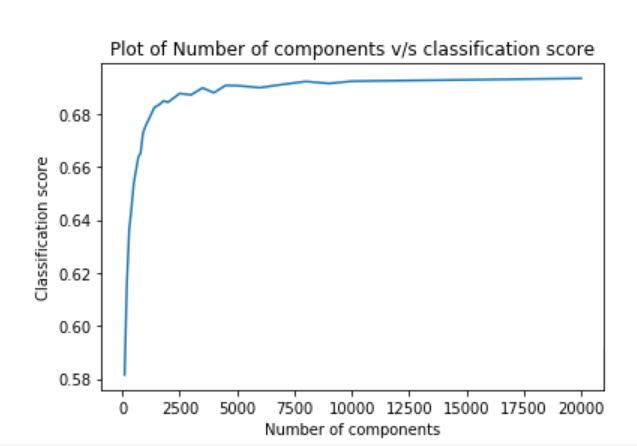
\includegraphics[scale=0.3]{figs/max_feat.png}
\caption{\label{fig:max_feat}The max-feature vs classification performances (acc) curve for the tf-idf vectorization. The optimal threshold is identified as $max\_feature \sim 5000$. The curve obtained for the "frequency count" method is analogous, and therefore omitted. }
\end{figure}
The results are reported in Fig.~\ref{fig:max_feat}, where an optimal cut-off threshold is identified in correspondence of $max\_feature = 5000$, i.e. only the first 5000 (frequency-wise sorted) features are kept. 
The same analysis is performed for both the "frequency count" and the "tf-idf" approaches, leading to overall similar results. 
Therefore, the same cut-off threshold is eventually chosen.

\item The latter analysis consists of a series of single value decompositions (SVD) with a different number of components kept. In particular, starting from the whole co-occurrence matrix (with frequency count, or with tf-idf score), with no cut-off thresholding applied, an attempt was made to reduce the feature dimensionality by means of the cited technique, by grid-searching the optimal number of components with respect to the final classification score (still performed with a RF model). 
\begin{figure}
\centering
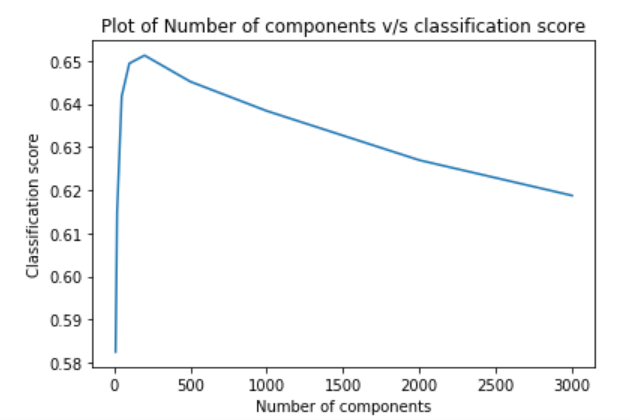
\includegraphics[scale=0.3]{figs/svd.png}
\caption{\label{fig:svd}The grid-search operation along with the number of components in the SVD process is plotted against the classification performances (acc), for the tf-idf vectorization. The optimal value for the number of components retained after the SVD is identified in correspondence of $\sim 300$. The curve obtained for the "frequency count" method has the same overall tendency, and therefore is omitted. }
\end{figure}
Fig.~\ref{fig:svd} reports the obtained curve, and when observing it two main conclusions can be drawn: first of all, an optimal number of components to keep after the SVD application seems to be almost $n\_components = 300$, and secondly, but importantly, the overall classification scores are systematically lower with respect to the first dimensionality-reduction approach (the cut-off threshold definition).
However, it is worth to notice that the SVD-reduced features are almost 100\% dense, and the classification phase reaches interesting performances with just 300 components. For a practical use on large scales, this could be very efficient. For the current project, given the fairly affordable computational cost even with the most effective approach (the cut-off threshold), we decided to select the cut-off method as the definitive BOW procedure, not relying anymore on the SVD approach.
\end{itemize}

Therefore, we identified the cut-off thresholding with $max\_feature = 5000$ as the most suitable configuration of the bag-of-words approach, relatively to the objective classification task.
This solution allows retaining effectiveness in the classification (i.e. the selected components seem not to significantly degrade the classification performances) and improves efficiency by reducing sparsity (the density of the initial feature vector, with no cut-offs, is estimated to be about $0.02 \%$ for both the BOW methods, whereas the final feature vectors density is estimated at almost $1.8 \%$, gaining an improvement of roughly two orders of magnitude.

\subsubsection{Word embedding \label{subsubsec:wordembedding}}
In order to use an alternative form of text representation compared to the more classic Bag of Words, it was decided to implement a word embedding approach.
Word embedding is the collective name for a set of language modeling and feature learning techniques in natural language processing (NLP) where words or phrases from the vocabulary are mapped to vectors of real numbers, is one of the most popular representations of document vocabulary and it is capable of capturing the context of a word in a document, semantic and syntactic similarity, relation with other words, etc.

In particular, for this project, three different approaches using word embedding have been undertaken exploiting two different predictive models such as \textbf{Word2Vec} and \textbf{Doc2Vec}.

Word2Vec (W2V) as described in \cite{word2vec} is a three-layer neural network, in which the first is the input layer and the last is the output layer while the middle layer builds a latent representation so the input words are transformed into the output vector representation. 
The ultimate goal of the model is to represent words in the vector space.
These models are highly efficient in understanding the context and relation between words. 
Similar words are placed close together in the vector space while dissimilar words are placed wide apart\footnote{Thanks to its properties, the representation through Word2Vec allows similar words to be represented by similar vectors, the vectors are decidedly less sparse than the Bag of Words representation and the relationship between the words is captured and maintained.}.
In particular, two models characterize W2V:
\begin{itemize}
\item Continuous Bag of Words (CBOW) in which the neural network takes a look at the surrounding words and predicts the word that comes in between;
\item Skip-grams with which the neural network takes in a word and then tries to predict the surrounding words.
\end{itemize}

Doc2Vec (D2V), on the other hand, computes a feature vector for each \textit{document} in the corpus and focuses on creating a document representation that should be good enough to predict the words in the document while W2V computes a feature vector for each \textit{word}.
Since, according to \cite{doc2vec}, D2V was created explicitly as an adaptation of W2V to the representation of entire documents as vectors rather than individual words, by the same authors, this too is divided into two models:
\begin{itemize}
\item Distributed Memory version of Paragraph Vector (PV-DM) acts as a memory that remembers what is missing from the current context or as the topic of the paragraph;
\item Distributed Bag of Words version of Paragraph Vector (PV-DBOW) is similar to W2V's skip-gram model.
\end{itemize}
\begin{figure}
\centering
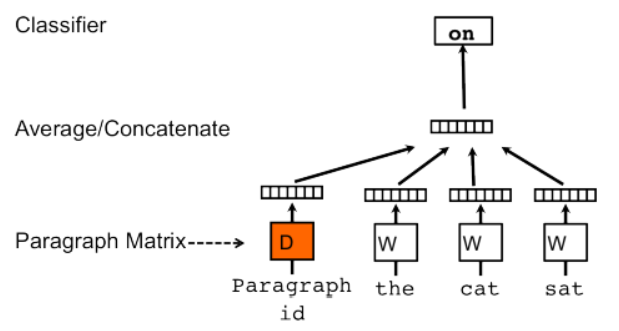
\includegraphics[scale=0.7]{figs/PV-DM.png}
\caption{PV-DM model representation. The diagram underlines how the D2V PV-DM model is substantially the W2V CBOW model with the addition of the Paragraph id vector.}
\label{fig:pvdm_model}
\end{figure}
In summary, the concept that the authors have used was simple: they have used the W2V model adding another vector (Paragraph id) so the model instead of using just words to predict the next word, use another feature vector, which is document-unique. An intuitive representation of this mechanism is reported in Fig.~\ref{fig:pvdm_model}

The three aforementioned approaches used for the word embedding text representation consist of two exploiting W2V and one D2V.

As said W2V map words into a vector representation, so using this characteristic a dictionary mapping word to a 300-dimensional vector was obtained. 
The choice of this precise dimensionality was guided by the desire to obtain a dense features representation.
The model chosen was a CBOW exploiting a window-size of 5 and trained using 10 epochs\footnote{It was verified that by increasing the number of epochs beyond 10, a better result was not obtained in the subsequent classification.}.
Subsequently, to exploit this representation to build features representing the entire documents two different strategies have been adopted:
\begin{itemize}
\item the simplest one requested to averaging word vectors for all words in a text, this particular representation has been named "W2V Mean";
\item the other exploits the Tf-idf weights representation and, for this reason, has been named "W2V Tf-idf".
\end{itemize} 

The last representation was obtained using D2V, in particular PV-DBOW because it resulted as the best model\footnote{In comparison with PV-DM and the cited in literature concatenation between the two models.}. 
Also, in this case, the model was trained only for 10 epochs. 
\subsection{Classification \label{subsec: classification}}
Once a series of different text representations has been obtained, including both Bag of Words as seen in Sec.~\ref{subsubsec:bow} and Word embedding in Sec.~\ref{subsubsec:wordembedding}, and considering the possibility of using four different results from the preprocessing pipeline, in particular using stemming/lemmatization and stemming plus badwords removal and lemmatization plus badwords removal as seen in Sec.~\ref{subsec:preprocessing} the focus shifted to the selection of some classification algorithms to maximize the performances.

The main objective of our approach was to compare a more classic machine learning (ML) model, technically simpler and computationally less expensive (for this reason several models were tested including Random Forest, Support Vector Machine and GradientBoosting) with a more complex deep learning (DL) approach, represented by the creation of a neural network (NN).

After several attempts, the best ML model for this specific task was identified in the Random Forest (RF) transversally to all preprocessing and text representation combinations, in good agreement with \cite{RF}. 
Random forest, consists of a large number of individual decision trees that operate as an ensemble and the fundamental concept behind RF is a simple but powerful one: the wisdom of crowds\footnote{A reason of why the random forest model works so well is because a large number of relatively uncorrelated models (trees) operating as a committee will outperform any of the individual constituent models.}. 

Following the selection, the RF hyper-parameters were also optimized exploiting a grid search optimization process which curiously led to the conclusion that the best value for the hyper-parameters was the default one.

As regards the NN instead, trying different architecture the best resulted in 3 dense layers with respectively 1024, 512 and 128 neurons with ReLU activation function, each one followed by a dropout layer with a rate of 50\%, concluding with an output layer with a number of neurons equal to the classification classes in combination with a Softmax activation function.

After several attempts, without going into detail as will be done in Sec.~\ref{sec:results}, the best model based on the classification performances turned out to be the NN, in particular using the vector representations created using D2V as features exploiting the texts treated with lemmatization and badwords removal.







\subsubsection{Optimization \label{subsubsec: optimization}}

\begin{table}[]
\centering
\begin{tabular}{ccc}
\hline
\multicolumn{1}{l}{Parameter} & Search Space                                                                              & \multicolumn{1}{l}{Final value} \\ \hline
n of neurons 1                & \begin{tabular}[c]{@{}c@{}}categorical\\ {[}64, 128, 256, 512, 1024, 2048{]}\end{tabular} & 1024                            \\
n of neurons 2                & \begin{tabular}[c]{@{}c@{}}categorical\\ {[}64, 128, 256, 512, 1024, 2048{]}\end{tabular} & 1024                            \\
n of neurons 3                & \begin{tabular}[c]{@{}c@{}}categorical\\ {[}64, 128, 256, 512, 1024, 2048{]}\end{tabular} & 128                             \\
dropout rate 1                & \begin{tabular}[c]{@{}c@{}}discrete uniform\\ {[}l = 0, h = 1, q = 0.1{]}\end{tabular}    & 0.1                             \\
dropout rate 2                & \begin{tabular}[c]{@{}c@{}}discrete uniform\\ {[}l = 0, h = 1, q = 0.1{]}\end{tabular}    & 0.5                             \\
dropout rate 3                & \begin{tabular}[c]{@{}c@{}}discrete uniform\\ {[}l = 0, h = 1, q = 0.1{]}\end{tabular}    & 0.0                             \\
activation function           & \begin{tabular}[c]{@{}c@{}}categorical\\ {[}LeakyReLU, ReLU{]}\end{tabular}               & ReLU                            \\
optimizer                     & \begin{tabular}[c]{@{}c@{}}categorical\\ {[}adam, Nadam, RMSprop{]}\end{tabular}          & Nadam                           \\
learning rate                 & \begin{tabular}[c]{@{}c@{}}loguniform\\ {[}l = 1e-4, h = 1e-4{]}\end{tabular}             & 0.00015                         \\ \hline
\end{tabular}
\caption{Summary representation of the hyper-parameters optimization search space: for each hyper-parameter subject to the optimization process the column "Search Space" contains the sampling method and the research area. The "Final value" column reports the values assumed by the hyper-parameters in correspondence with the best value obtained by the objective function during the optimization process.}
\label{tab:optimization_search_space}
\end{table}

\begin{figure}
\centering
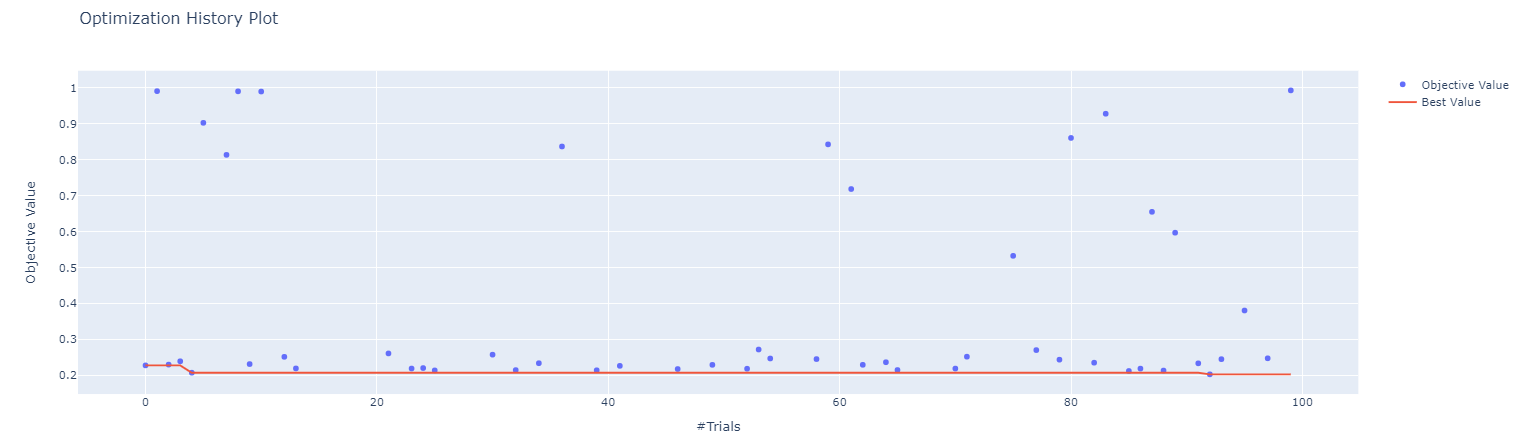
\includegraphics[scale=0.45]{figs/optimization_best_seen.png}
\caption{Visualization representing the best-seen development during the 100 evaluations for the optimization task: while the blue points represent the value obtained from the objective function for each evaluation, the red line follows the best results. The output of the objective function is the Macro F-Measure error obtained through 5-folds cross-validation.}
\label{fig:optimization_best_seen}
\end{figure}
As anticipated in Sec.~\ref{subsec: classification}, the model that has achieved the highest performances among the various tested, considering also the different combinations of preprocessing and text representation, is the one comprising the neural network with as input the features obtained from the representation through D2V of the documents treated through lemmatization and the badwords removal.

Aiming to optimize the hyper-parameters of the neural network, a Bayesian optimization framework was used combining Optuna and Scikit-Optimize exploiting the Random Forest as a surrogate model and the Lower Confidence Bound as the activation function.
To obtain an optimization as robust as possible, 100 evaluations have been performed without using fixed seeds and performing, inside each evaluation, a 5-folds cross-validation.
The choice of this particular framework was determined by the fact that it is very performing. In fact, it allows to:
\begin{itemize}
\item use a SQL server as history storage so that it is possible to perform the optimization at different times without losing the data;
\item activate a native pruning mechanism which allows saving a lot of time during the various evaluations, discarding a priori the attempts that immediately prove to be unpromising compared to those previously made;
\item produce a series of helpful representations in a Plotly\footnote{\url{https://plot.ly/python/}} fashion useful for monitoring the progress of the optimization.
\end{itemize} 
In particular, the focus of the optimization was the number of neurons of the dense layers, the intensity of the regularization given by the rate of the dropout layers, the choice of the optimizer with its learning rate and the activation function to use between each layer: a summary of the optimized hyper-parameters together with their search space is available in Tab.~\ref{tab:optimization_search_space}.
In Fig.~\ref{fig:optimization_best_seen} it is possible to observe the trend of the best-seen during the optimization process. In particular, what is minimized is
\begin{equation}
1-\text{Average macro F-measure}
\end{equation}
where average means the average of the five values of macro F-measure derived from the usage of a 5-folds cross-validation into the objective function.



\section{Results and Evaluation \label{sec:results}}

\subsection{Best Processing Method with respect to Text Representation}
A comparison of the different preprocessing methods described in Sec.~\ref{subsec:preprocessing} in combination with the various text representation introduced in Sec.~\ref{subsec:text-prepresentation} is performed, aiming to identify, for each representation, which method is the most suitable for the given classification problem. The classifier exploited for the initial comparison is the Random Forest, due to its proven stability and efficiency, resulting in fast classification phases.

The results of this procedure are reported in Tab.~\ref{tab:evaluations}. In particular, the "Stemming + Badwords Removal" method reveals to be suitable both with the "Tf-idf" and the W2V text representations, whereas the "Lemmatization + Badwords Removal" processing turns out to be the most effective in correspondence with the representations given by both frequency-count and Doc2Vec.
It is worth to notice that the procedure of "Badwords Removal", implemented throughout the LDA analysis, reveals to be effective in both the applied cases, increasing the general classification performance measures by up to $\sim 1\%$.

\begin{table}[]
\resizebox{\textwidth}{!}{
\begin{tabular}{ccccccccccccc}
\hline
\multicolumn{1}{l}{Processing method}         & \multicolumn{3}{c}{Stemming}                 & \multicolumn{3}{c}{Stemming+Badwords Removal} \\
\multicolumn{1}{l}{Feature Extraction Method} & Acc   & Macro F-Measure & Weighted F-Measure & Acc    & Macro F-Measure & Weighted F-Measure \\ \hline
Count                                         & 0.692 & 0.659           & 0.687              & 0.692  & 0.659           & 0.687\\
Tf-idf                                        & 0.689 & 0.656           & 0.685              & \textbf{0.691}  & \textbf{0.660}            & \textbf{0.686}  \\
W2V Tf-idf                                    & 0.679 & 0.639           & 0.675              & \textbf{0.683}  & \textbf{0.648}           & \textbf{0.680}  \\
W2V Mean                                      & 0.668 & 0.621           & 0.663              & \textbf{0.677}  & \textbf{0.637}           & \textbf{0.674}  \\
Doc2Vec                                       & 0.735 & 0.727           & 0.735              & 0.743  & 0.737           & 0.743  \\ \hline
\end{tabular}
}
\newline
\vspace{1mm}
\newline
\resizebox{\textwidth}{!}{
\begin{tabular}{ccccccccccccc}
\hline
\multicolumn{1}{l}{Processing method}     & \multicolumn{3}{c}{Lemmatization}            & \multicolumn{3}{c}{Lemmatization+Badwords Removal} \\
\multicolumn{1}{l}{Feature Extraction Method} & Acc   & Macro F-Measure & Weighted F-Measure & Acc    & Macro F-Measure & Weighted F-Measure \\ \hline
Count   & 0.692 & 0.661           & 0.687              & \textbf{0.693}   & \textbf{0.662}             & \textbf{0.688}                \\
Tf-idf                & 0.688 & 0.656           & 0.684              & 0.688   & 0.658             & 0.684                \\
W2V Tf-idf                  & 0.682 & 0.641           & 0.678              & 0.683   & 0.644             & 0.679                \\
W2V Mean                & 0.670  & 0.623           & 0.665              & 0.674   & 0.631             & 0.670                 \\
Doc2Vec                                                     & 0.746 & 0.742           & 0.746              & \textbf{0.750}    & \textbf{0.745}             & \textbf{0.750}                 \\ \hline
\end{tabular}
}
\caption{Summary of the evaluation procedure applied. Each preprocessing method is combined with each text representation procedure and is evaluated using Accuracy, Macro F-Measure, and Weighted F-Measure exploiting RF as a classification model. The choice of evaluation metrics lies in the need to obtain weighted measurements with respect to the imbalance of the different classes.}
\label{tab:evaluations}
\end{table}


\subsection{Best Text Representation and Classification Model}
After the initial comparison, another evaluation process is carried out in order to identify the most suitable text representation and the best machine learning classifier. 
The various text representations are evaluated in correspondence with the best processing methods selected in the previous section.
After an initial general investigation regarding the suitable classification algorithms mentioned in Sec.~\ref{subsec: classification}, the RF and the NN are chosen to be compared in a 5-folds CrossValidation procedure.
The comparison is reported in Tab.~\ref{tab:results}, where the combination of the "Lemmatization + Badwords Removal" preprocessing method, the text representation given by the Doc2Vec algorithm with the NN classifier, which clearly outperforms the other possible combinations.
Therefore, the contribution of the Doc2Vec representation seems to be crucial when explaining the highest obtained result. 
Clearly, the highly specialized document representation provided by such an algorithm reveals to be the most suitable approach in our difficult classification problem, where the similarity among some categories, and therefore among their most representative words, strongly influences the performance of BOW and "single" word-embedding methods.
In is worth to notice that, besides the good behaviour of Doc2Vec, there is no great distinction in performances when considering the other investigated text representation.
\begin{table}[]
\resizebox{\textwidth}{!}{
\begin{tabular}{ccccccccccc}
\hline
\multicolumn{3}{l}{}                                                                   & \multicolumn{2}{c}{Acc.} & \multicolumn{2}{c}{Top-3 Acc.} & \multicolumn{2}{c}{Macro F-Meas.} & \multicolumn{2}{c}{Weighted F-Meas.} \\
\multicolumn{1}{l}{Model} & Processing method              & Feature Extraction & value      & std        & value         & std           & value            & std              & value              & std               \\ \hline
NN                        & Lemm.+BR & Count                     & 0.693      & 0.002      & 0.907         & 0.001         & 0.673            & 0.004            & 0.693              & 0.002             \\
NN                        & Stemm.+BR      & Tf-idf                    & 0.692      & 0.003      & 0.908         & 0.001         & 0.671            & 0.003            & 0.691              & 0.003             \\
NN                        & Stemm.+BR      & W2V Tf-idf                & 0.695      & 0.002      & 0.901         & 0.001         & 0.678            & 0.002            & 0.693              & 0.002             \\
NN                        & Stemm.+BR      & W2V Mean                  & 0.692      & 0.003      & 0.901         & 0.002         & 0.671            & 0.005            & 0.690               & 0.004             \\
NN                        & Lemm.+BR & Doc2Vec                   & \textbf{0.784}      & 0.002      & \textbf{0.941}         & 0.001         & \textbf{0.796}            & 0.001            & \textbf{0.784}              & 0.002             \\
RF                        & Lemm.+BR & Count                     & 0.693      & 0.004      & 0.865         & 0.002         & 0.663            & 0.005            & 0.689              & 0.004             \\
RF                        & Stemm.+BR      & Tf-idf                    & 0.693      & 0.004      & 0.865         & 0.002         & 0.664            & 0.005            & 0.689              & 0.004             \\
RF                        & Stemm.+BR      & W2V Tf-idf                & 0.685      & 0.001      & 0.870         & 0.001         & 0.650             & 0.002            & 0.682              & 0.001             \\
RF                        & Stemm.+BR      & W2V Mean                  & 0.678      & 0.002      & 0.874         & 0.001         & 0.638            & 0.004            & 0.674              & 0.002             \\
RF                        & Lemm.+BR & Doc2Vec                   & 0.751      & 0.003      & 0.911         & 0.001         & 0.746            & 0.003            & 0.751              & 0.003             \\ \hline
\end{tabular}
}
\caption{Summary of the final results obtained through 5-folds cross-validation. The best Processing Method obtained from the evaluation procedure has been combined with the corresponding best Feature Extraction Method for both the classification models. The chosen metrics are classic Accuracy, Top-3 Accuracy, where the correct class only needs to be in the top three predicted classes to positively count in the classification, Macro F-Measure and Weighted F-Measure. Exploiting the CV procedure each metric is reported with its mean value and standard deviation between the five surveys.}
\label{tab:results}
\end{table}



\subsection{Final Results and Error Analysis}
\begin{figure}
\centering
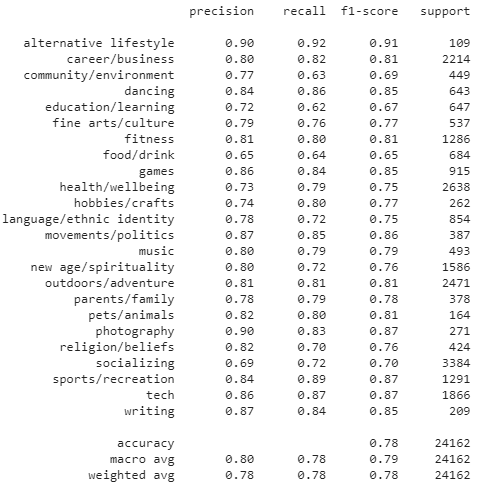
\includegraphics[scale=0.9]{figs/classification_report.png}
\caption{Classification report of the final model (NN with Lemm.+BR and D2V representation) after the optimization procedure.}
\label{fig:classification_report}
\end{figure}

Considering the best-developed model (NN + Lemm.+BR + D2V), a detailed report in terms of classification performances for the single classes is visualized in Fig.~\ref{fig:classification_report}. 

\begin{figure}
\hspace{-1cm}
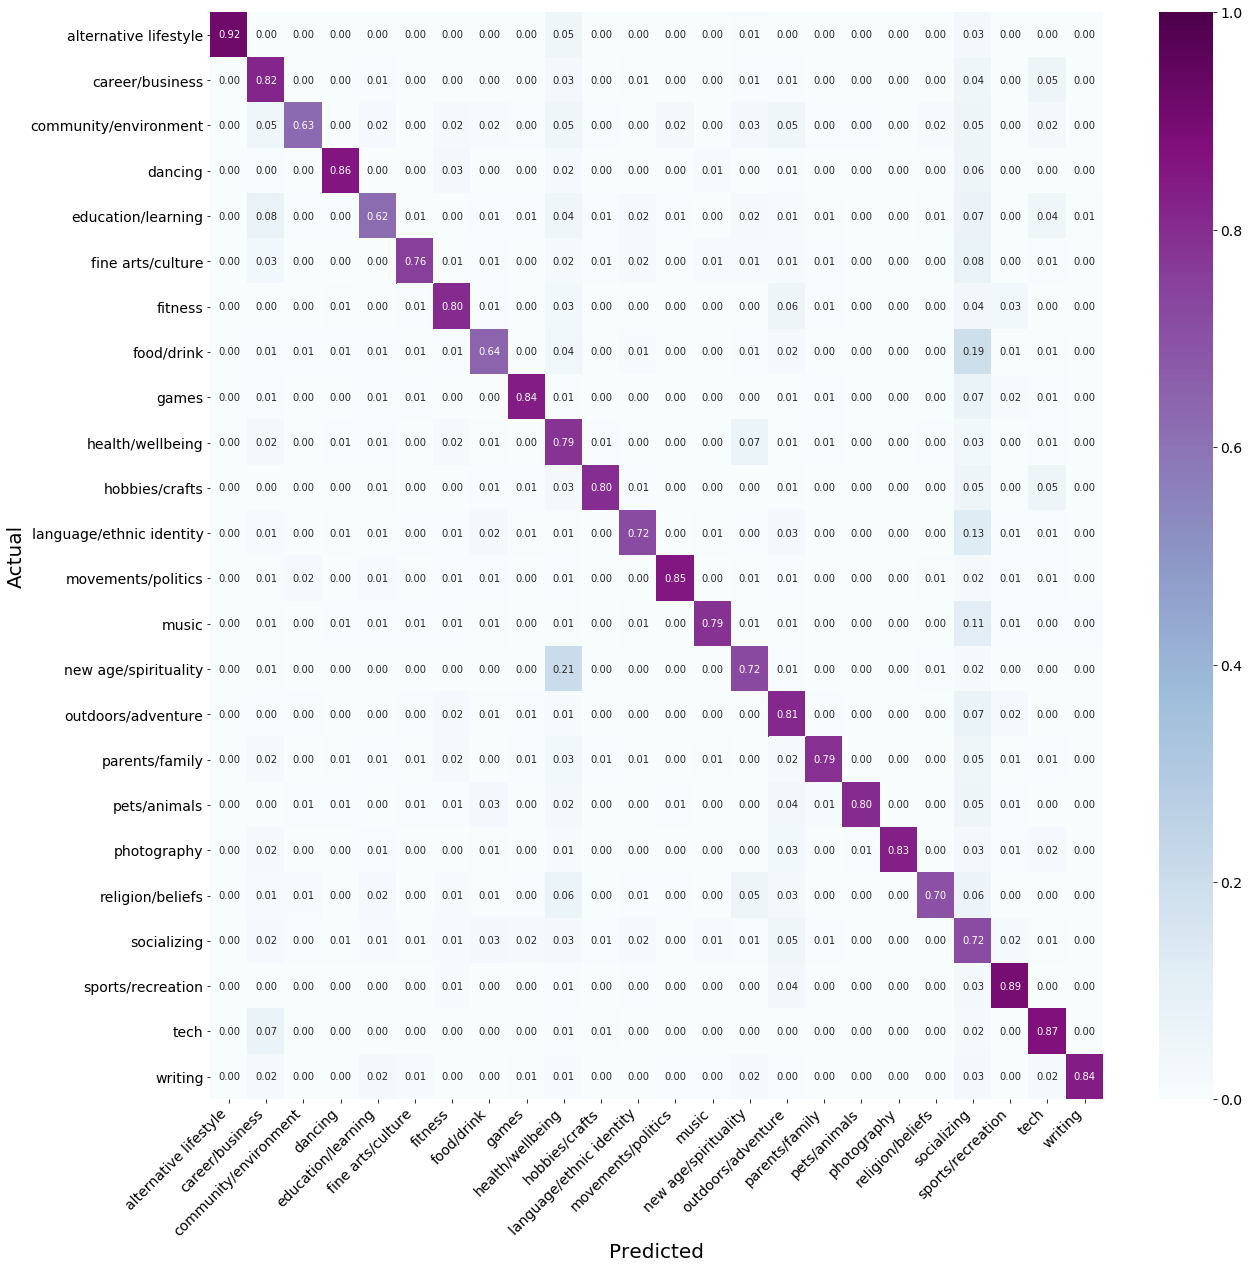
\includegraphics[scale=.4]{figs/plot_confusion_matrix.png}
\caption{Heatmap fashion representation for the confusion matrix of the final model (NN with Lemm.+BR and D2V representation). The absolute frequencies have been normalized with respect to the row sum, obtaining the Recall measure on the diagonal.}
\label{fig:confusion_matrix}
\end{figure}

As additional support for precise error analysis, the confusion matrix obtained is shown is Fig.~\ref{fig:confusion_matrix}. 
It is worth to notice that the most confusing category is "socializing", since different others are misclassified as "socializing". 
This phenomenon is explained considering the generality of the topic represented by the category, whose most representative words are intuitively associated with those characterizing other categories, such as "food/drink".
Another example of misclassification can be identified considering that "new age/spirituality" is slightly confused with "health/wellbeing". Indeed, many meetup-groups treating the well-being topic are very similar to those interpreting the spirituality investigation as a way to a better/more relaxed life.

\section{Conclusions and Improvements}

During some previous projects developed around Meetup.com data, the need to categorize the events according to their topics and based on their descriptions arose. Therefore, a typical text-mining pipeline is applied to a labelled Meetup.com event description dataset, in order to enable a text (description) single-label multi-class (24 classes) classification task.
Different preprocessing methods are initially compared against text representations provided by various methods (BOW, Word-embedding) and tested with different classifiers (RF, NN).
The most performant procedure turns out to be a preprocessing based on Lemmatization (plus "badwords removal") followed by classification through a NN performed over the text representation obtained with the D2V algorithm. 
The resulting classification performances asses about a $top-1 acc. = 0.784$ and a $top-3 acc = 0.941$, which reveals to be a quite satisfying performance especially considering the relatively high number of target classes.
This method seems to outperform the other combinations by far. 
The result is explained in terms of the capability of D2V, being an unsupervised algorithm specifically designed for document-embedding, to better discriminate the content of the corpus not being so much influenced by the similarity among some classes, which typically penalize the W2V word-embedding and the BOW approaches.

Possible improvements could be identified among the gathering of more data, especially from the under-represented categories, performing a more in-depth LDA analysis, systematically varying the number of produced clusters (topics), in order to better select the "badwords" (stop-words for the given problem). Another interesting improvement could be to exploit the "BERT" algorithm, developed by Google, to create possibly even better embeddings with respect to D2V.


\section*{Acknowledgements}
We would like to thank the Professors G. Pasi and M. Viviani for their support during the development of the project.

\begin{thebibliography}{9}

\bibitem{lda}
D. M. Blei, A. Y. Ng, and M. I. Jordan, (2003). "Latent dirichlet allocation", The Journal of Machine Learning Research, 3, 993-1022.

\bibitem{word2vec}
T. Mikolov, G.s Corrado, K. Chen, J. Dean, (2013). "Efficient Estimation of Word Representations in Vector Space", ICLR 2013, 1-12.

\bibitem{doc2vec}
Q. Le and T. Mikolov , (2014). "Distributed Representations of Sentences and Documents", Proceedings of the 31st International Conference on Machine Learning, in PMLR, 32(2), 1188-1196.

\bibitem{RF}
D. Xue and F. Li, (2015). "Research of Text Categorization Model based on Random Forests", IEEE International Conference on Computational Intelligence \& Communication Technology, 173-176.

\end{thebibliography}

%\begin{appendix}
%\appendix
%\section{Appendix: model details, code and data\label{sec:appendix}}

%\end{appendix}
\end{document}
